
\chapter{多视图几何基础}
\section{相机成像模型}


\section{相似变换、仿射变换、射影变换的区别}
\textbf{相似变换}。就是在刚体变换的基础上加了一个尺度因子,刚体变换是保距离和角度的变换,那么相似变换不保距离,但是保角度,保平行。

\textbf{仿射变换}。不保角度,保平行

\textbf{射影变换}。






\section{各种矩阵的区别}


单应矩阵,9个元素,因为相差一个尺度因子,所以自由度为8.那么为什么会相差一个尺度因子呢?因为单应矩阵变换时是作用在齐次坐标系下的,所以单应矩阵乘以一个任意非0的尺度因子,其得到的结果都是一样的。

基础矩阵,9个元素,因为相差一个尺度因子,并且基础矩阵的行列式为0(因为基础矩阵是奇异矩阵,为什么呢?因为基础矩阵1个点对应1条线,而不是1个点对应1个点),所以基础矩阵的的自由度为7。

本质矩阵,9个元素,5个自由度,旋转具有3个自由度,平移矩阵2个自由度(本来平移矩阵3个自由度,但是本质矩阵相差一个尺度因子),所以变成了两个自由度。


\section{单应矩阵和基础矩阵的应用场景}

单目相机进行初始化时,如果场景是平面、近似平面或低视差(low parallax)的场景,那么需要用\textbf{单应矩阵}进行初始化,非平面场景且视差足够大的情况下,需要使用\textbf{基础矩阵}进行初始化。

需要搞清楚为什么,就需要解决如下的两个问题:
\begin{enumerate}
	\item 为什么基础矩阵不能应用于平面场景
	\item 为什么单应矩阵不能应用于非平面场景。
\end{enumerate}


下面将依次介绍\textbf{纯旋转下单应矩阵和基础矩阵的区别},\textbf{平面场景下的基础矩阵}和\textbf{非平面场景下的单应矩阵}。

\subsection{纯旋转下的单应矩阵和基础矩阵}

基础矩阵的计算公式如下:
\begin{equation}
	F = K^T[t]_x RK
\end{equation}
可以看出,纯旋转的情况下,基础矩阵会挂掉,因为平移是0。所以纯旋转的情况下,不能够使用基础矩阵。或者从另一个方面来认知,对极几何必须要相机光心之间的基线不为零才有的,因此在纯旋转平移为零的情况下,自然是没有对极几何存在的,也就不能使用基础矩阵了。



在已知旋转和平移的情况下,单应矩阵的计算公式如下:
\begin{equation}
	H = R - tn^T/d
\end{equation}


在纯旋转$t = 0$的情况下, 可以发现矩阵$H$和深度$d$没有关系了,无论三维点是否在一个平面上,矩阵$H$都能符合它们之间的转换关系。又或者可以这样思考,每个3D点都在一个平面上(不同的3D点可以在相同或不同的平面上),平面通过$n$和$d$参数化,将其带入到公式中,由于在纯旋转的情况下,不管$n$和$d$是什么,求出来的单应矩阵$H$都是一样的,所以纯旋转的情况下能够使用单应矩阵。





\subsection{平面场景下的基础矩阵}


\textbf{为什么基础矩阵不能应用于非平面场景}。基础矩阵的计算公式如下:
\begin{equation}
	F = K^T[t]_x RK
\end{equation}
可以看出,纯旋转的情况下,基础矩阵会挂掉,因为平移是0,不过这不是重点。下面来推导为什么基础矩阵不能用于平面场景。假设场景是平面且能够使用基础矩阵,那么就有如下两个公式:
\begin{equation}
	x' = Hx
\end{equation}
\begin{equation}
	x^TFx' = 0
\end{equation}

将$x' = Hx$带入到公式$x^TFx'=0$中,得到:
\begin{equation}
	x'FHx = 0
\end{equation}
可以看到这个一个二次型,二次型为0,那么二次型矩阵是反对称矩阵,也就是说只要矩阵$FH$是一个反对称矩阵,这个等式就永远成立,也就是说求得的基础矩阵并不唯一(这可不是尺度不确定的那种不唯一)。并且反对称矩阵只有3个自由度,

\begin{note}
但是这也只能说明$FH$只有3个自由度,而不能说明$F$只有3个自由度,也不能说明基础矩阵$F$退化啊。
\end{note}


\subsection{非平面场景下的单应矩阵}

单应矩阵的公式如下:
\begin{equation}
	H = R - tn^T / d
\end{equation}

假设场景是非平面的,然后我们通过RANSAC算法估计了一个满足大多数点对应情况的单应矩阵。那么也就是说我们拟合了一个潜在的平面(其参数为$n$和$d$),如图\ref{fig:nonplanar_homography}所示。所以我的理解是,在使用RANSAC+DLT方法计算单应矩阵时(随机选择4个点),就相当于隐式地计算了潜在平面的参数$n$和$d$。然后在计算内点时,就是要找到误差比较小的点,那么理论上应该是那些距离潜在平面比较近的点,因为对应那些不在平面上的3D点所对应的2D点(左图像上的点),利用单应矩阵转换之后,会强迫其落在潜在平面上,然后再投影到右平面上。这个过程中,离平面近的点产生的误差比较小,而离平面较远的点产生的误差比较大。所以在使用RANSAC+DLT算法求解单应矩阵时,应该就是在3D空间中找到一个平面,使得该平面周围的点尽可能多。


所以说,在非平面场景下使用单应矩阵时,如果特征点所对应的3D点中存在这样一个满足大多数点的平面,那么求得的单应矩阵所对应的内点就多,否则内点数就少。

\begin{note}
	以上的推导纯粹我自己的理解,并不一定正确,因为推导的使用并没有将旋转平移也考虑在内。而且我的这个推导并不能解决\textbf{低视差}情况下能够使用单应矩阵。
\end{note}

\begin{figure}[h]%%图
	\centering  %插入的图片居中表示
	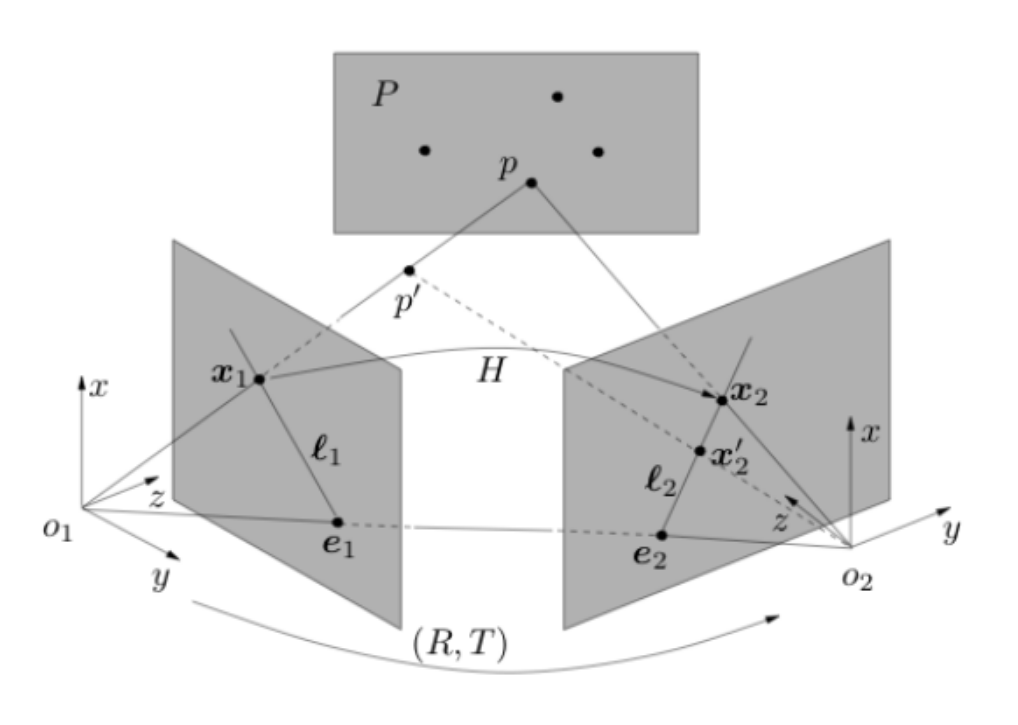
\includegraphics[width=0.6\linewidth]{image/Multiview-Geometry-Base/nonplanar_homography.png}  %插入的图,包括JPG,PNG,PDF,EPS等,放在源文件目录下
	\caption{非平面场景下的单应矩阵.}  %图片的名称
	\label{fig:nonplanar_homography}   %标签,用作引用
\end{figure}



\section{各种矩阵计算}






单应矩阵,DLT
基础矩阵,8点法,7点法
本质矩阵,8点法,5点法

\section{位姿计算}
\subsection{2D-2D}
本质矩阵分解
单应矩阵分解
\subsection{2D-3D}
PnP
\subsection{3D-3D}
3D-3D变换

\section{三角测量}

